\section{Artefact}\label{sec:artefact}

The model is a combination the microeconomic and macroeconomic.

As it deals with processes off the small scale, e.g., there is one delivery company, one supply and demand market (i.e., the deliverers labour marker), and
individual agents.



More macroeconomic elements could be added in future versions, e.g., unexpected events like COVID pandemic which created a peak in food ordering.


The conceptional model has 3 types of agents:

-deliverers \\
-restaurants \\
-customers \\

There is one orchestrator, the delivery company, offers a website where customers can order,
restaurants pay the company a percentage of the delivery, they also offer means for the deliverers to
find deliveries and the shortest route.

Everything works on ticks of the clock, during 1 tick all agents execute one behavior rule.
The order of execution among agents of one type is arbitrary.
This is interleaved execution, no parallelism.

%In the real world when ordering food, a customer will use the website from the delivery company to find a restaurant and place an order.
%The restaurant will take the order, the app
% Short telling how it works in the real world, Youtube

deliverers:
Start number can be set.
The deliverers get


restaurants:
the start number can be set, are placed at random
accept any orders, are open all the time,
prepare meals, the preparation time can be set,
after accepting a deliverer is asked.
when the meal is ready it can be picket up.
Restaurants will leave the system if they have not enough orders.

customers:
order distribution, peek ours breakfast, lunch and  diner, once a week.
order from any restaurant they have no bad experience with
the price distribution, average can be set
they remember bad experiences for a certain time.
If delivered stale the customer is not satisfied and will not order from the restaurant also
it will order less food per week.

\begin{figure}
    \centering
    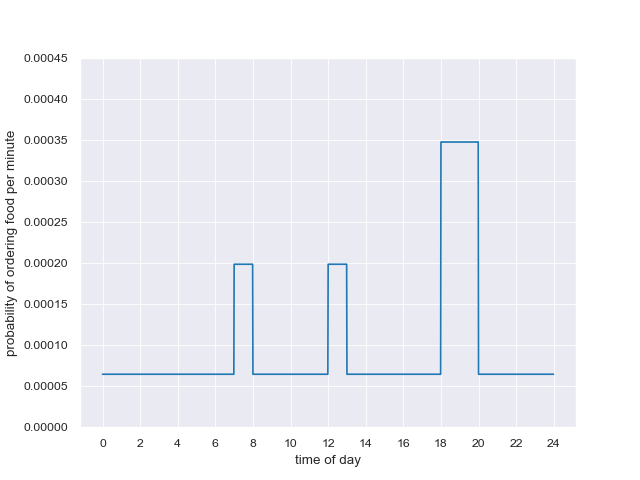
\includegraphics[width=9cm]{sections/pics/food_ordering_distribution}
    \caption{Food ordering probablities for one day}
    \label{fig:food_ordering_distribution}
\end{figure}



meals:
meals have properties, stage: ordered , ready, in\_transit, delivered, expired
A meal is only fresh for a time period.
If not picked up it wil be discarded.





\begin{itemize}
    \item   The world consists op a grid of squares, some squares will be blocks of buildings and others represent the streets.
    \item   On this grid some predetermined restaurants and customers exist.
    \item   Customers will order food at a restaurant, the restaurant will prepare the food en will ask for a deliverer.
    \item   A deliverer will claim the delivery, move to the restaurant, pick the food up and move to the customer.
    \item   Agents may leave the world, i.e.,choose another delivery company, when unhappy.
    \item   Unhappiness will occur:
    \begin{itemize}
        \item   for customers when the food is not or too late delivered,
        \item   for restaurants when the food is not picked up or no orders are being placed,
        \item   for deliverers when they don't make any money.
    \end{itemize}
    \item    Calculating the profit for the delivery company.
    \item    The simulation consists of discreet steps, in which all agents simultaneous can do one thing.
    Some examples are:
    \begin{itemize}
        \item  move to the next square
        \item  place an order at a restaurant
        \item  do nothing
        \item  decide to take an order
    \end{itemize}
    \item   Behavior of the agents is rule based, these have to be programmed.
\end{itemize}


The environment where multiple agents act is called a multi-agent system end the problem is called a multi-agent planning problem (from~\cite{russell2016artificial}).
The research problem is actually a comparison between a system where there is one decision maker (the company assigns delivery jobs) and a system where each deliverer decide for its self (multiple decision makers).
This research will not be of a thoroughly theoretical nature though, its more of an exploratory/explanatory nature, see what happens under some conditions and explain the correlation.

\begin{figure}
    \centering
    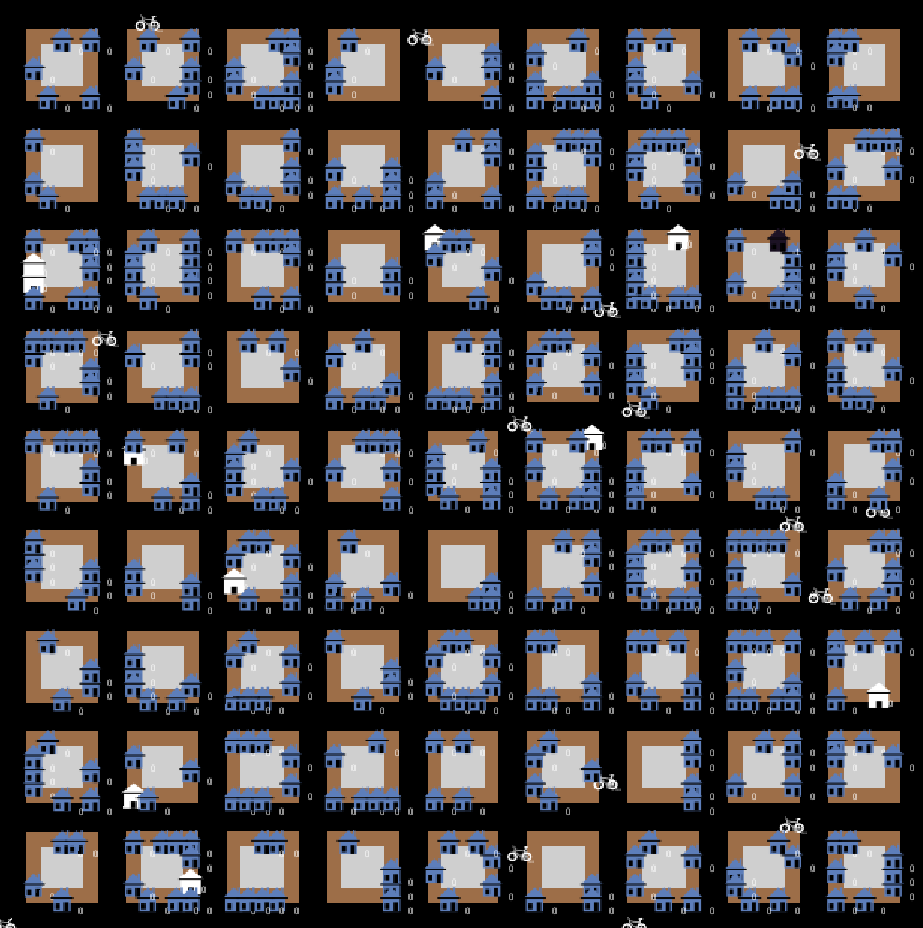
\includegraphics[width=9cm]{sections/pics/grid}
    \caption{Fooddelivery grid}
    \label{fig:grid}
\end{figure}

\begin{figure}
    \centering
    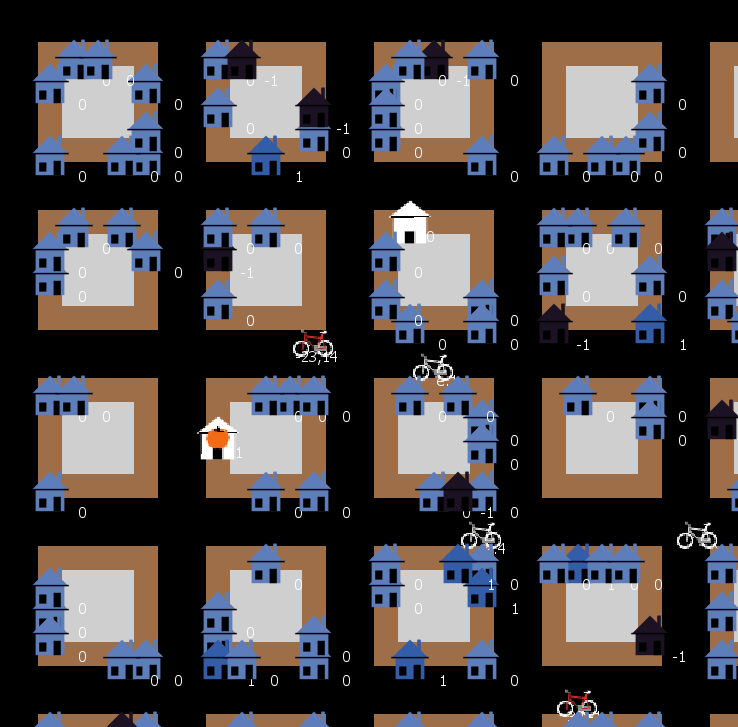
\includegraphics[width=9cm]{sections/pics/grid_closeup}
    \caption{Fooddelivery grid closeup}
    \label{fig:grid closeup}
\end{figure}


\begin{figure}
     \centering
     \begin{subfigure}[m]{0.1\textwidth}
         \centering
         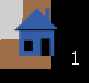
\includegraphics[width=\textwidth]{sections/pics/cust_happy}
         \caption{Customer with happyness score}
     \end{subfigure}
     \hfill
     \begin{subfigure}[m]{0.1\textwidth}
         \centering
         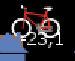
\includegraphics[width=\textwidth]{sections/pics/del_on_its_way}
         \caption{Deliverer on route to loc 23,1}
     \end{subfigure}
     \hfill
     \begin{subfigure}[m]{0.1\textwidth}
         \centering
         
\includegraphics[width=\textwidth]{sections/pics/meal_prep}
         \caption{Restaurant with meal ordered on top and number of ordered}
     \end{subfigure}
      \hfill
     \begin{subfigure}[m]{0.1\textwidth}
         \centering
         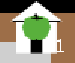
\includegraphics[width=\textwidth]{sections/pics/meal_ready}
         \caption{Restaurant with meal ready on top and number of ordered}
     \end{subfigure}
        \caption{Agents examples}
        \label{fig:agents}
\end{figure}






\section{Results of simulations}\label{sec:results-of-simulations}


Consumers order meals from restaurants they like, if a meal is delivered cold they dislike the restaurant.
If they dont like the restaurant they will not place any orders anymore at that restaurant.

Restaurants create meals, if they dont get any orders for some time they quit.

The delivery provider make money for each order placed via their system, at the end they must have enough deliverers so that
customers keep ordering.
They have to pay the deliverers for the deliveries.



\subsection{Model variant 1}
Here come the results belonging to variant where deliverers are hired and paid an hourly wage.
The company destributes deliveries equally among the hired employees.
The company has to deside on how many to hire and for which periods.


\subsection{Model variant 2}
Here come the results where deliverers are independent contractors.
Deliverers come and go whenever they are pleased, like a open market.
Now deliverers have to deside to become a deliverer, deside to stop and to decide to go for a delivery.
To keep this simple, the meals are destributed among the available deliverers.
If a delivery person does not make enough many during a day they will quit.
